\documentclass[a4paper]{article}
\usepackage[a4paper]{geometry}
\usepackage{amsmath}
\usepackage{amssymb}
\usepackage[utf8]{inputenc}
\usepackage{graphicx}
\usepackage{booktabs}
\usepackage[russian]{babel}
\usepackage{flafter}
\usepackage{caption}

\title{Лабораторная работа 2.1.4 \\Определение теплоёмкости твёрдых тел}
\date{02 мая 2017 г.}
\author{Вячеслав Ждановский, студент 611 группы ФРКТ\\
Шамиль Вагабов, студент 611 группы ФРКТ\\
Станислав Токарев, студент 611 группы ФРКТ}
\begin{document}
	\pagenumbering{gobble}
	\maketitle
	\newpage
	\pagenumbering{arabic}
	\paragraph{Цель работы:} 1) измерение кол-ва подведённого тепла и вызванного им нагрева твёрдого тела. 2) определение теплоёмкости поо экстраполяции отношения $\frac{\Delta Q}{\Delta T}$ к нулевым потерям теплам. 
	\paragraph{В работе используются:} 
	калориметр с нагревателем и термометром сопротивления; амперметр; вольтметр; мост постоянного тока; источник питания 36V.
	\paragraph{Cхема установки:}
	\begin{figure}[ht!]
		\centering
		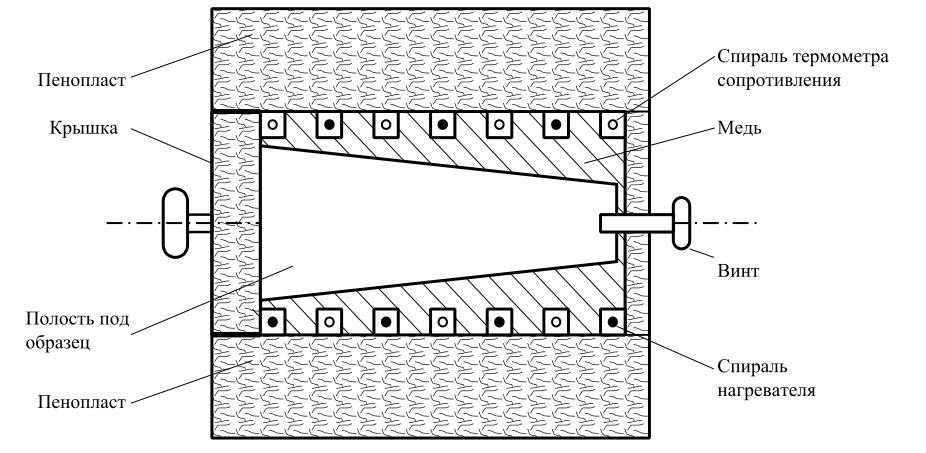
\includegraphics[height=60mm]{pic1.png}
		\caption{Схема устройства калориметра}
	\end{figure}
	\begin{figure}[ht!]
		\centering
		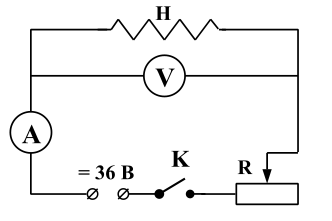
\includegraphics[height=45mm]{pic2.png}
		\caption{Схема включения нагревателя}
	\end{figure}
	Установка состоит из калориметра с пенопластовой изоляцией, помещённого в ящик из многослойной клееной фанеры. Внутренние стенки калориметра выполнены из материала с высокой теплопроводностью. Надежность теплового контакта между телом и стенками обеспечивается их формой: они имеют вид усечённых конусов и плотно прилегают друг к другу. Для выталкивания образца служит винт в донышке внутренней стенки калориметра. В стенку калориметра вмонтирован электронагреватель и термомтер сопротивления. Схема включения нагревателя изображена на рисунке 2. \\
	Система реостатов позволяет установить нужную силу тока в цепи нагревателя. По амперметру и вольтмерту определяется мощность, выделяемая током в нагревателе. Величина сопртивления термометра измеряется мостом постоянного тока. 
	\paragraph{Необходимая теория}
	В предлагаемой работе измерение теплоёмкости твердых тел производится по обычной схеме. Исследуемое тело помещается в калориметр. Измеряется $\Delta Q$ - количество тепла, подведённого к телу и $\Delta T$ - изменение температуры тела, произошедшее в результате подвода тепла. Теплоёмкость определяется по формуле
	\begin{equation}
	C=\frac{\Delta Q}{\Delta T}
	\end{equation}
	Температура исследуемого тела надёжно измеряется термометром (в нашем случае - термометром сопротивления), а определение кол-ва тепла, поглощённого телом, вызывает затруднение. В реальных условиях не вся энергия $P\Delta t$, выделенная нагревателем на нагревание исследуемого тела и калориметра, часть её уходит из калориметра благодаря теплопроводности его стенок. Оставшиеся в калориметре кол-во тепла $\Delta Q$ равно:
	\begin{equation}
	\Delta Q = P\Delta t - \lambda(T-T_k) \Delta t
	\end{equation}
	где $P$ - мощность нагревателя, $\lambda$ - коэффициент теплоотдачи стенок калориметра, $T$ - темпераутра тела, $T_k$ - темпераутра окружающего калориметр воздуха (комнатная), $\Delta t$ - время, в течение которого идет нагревание. 
	Из уравнений (1) и (2) получаем
	\begin{equation}
	C=\frac{P - \lambda(T-T_k)}{\Delta T/\Delta t}
	\end{equation}
	Формула (3) является основной расчётной формулой работы. Она определяет теплоёмкость тела вместе с калориметром. Теплоёмкость калориметра должна быть измерена отдельно и вычтена из результата. С увеличением температуры исследуемого тела растёт утечка энергии, связанная с теплопроводностью стенок калориметра. Погрешности, связанные с утечкой тепла, оказываются небольшими, если не давать телу заметных перегревов и поизводить все измерения при температурах, мало отличающихся от комнатной ($T \rightarrow T_k$).
	Однако при небольших перегревах возникает большая ошибка в измерении $\Delta T = T - T_k$. Чтобы избежать этого, зависимость скорости нагревания $\Delta/\Delta t$ от температуры измеряется в широком интервале изменения температур. По полученным данным страится график:
	\begin{equation}
	\frac{\Delta T}{\Delta t} = f(T)
	\end{equation}
	который экстраполируется к температуре $T=T_k$, и, таким образом, определяется скорость нагревания при комнатной температуре. Подставляя полученное выражение в формулу (3) и, замечая что при $T=T_k$, член $\lambda (T-T_k)=0 \implies$
	\begin{equation}
	C=\frac{P}{(\Delta T/\Delta t) T_k}
	\end{equation}
	Температура измеряется термометром сопротивления, представляющим собой медную проволоку, намотанную на теплопроводящий каркас внутренней стенки калориметра (рис 1). Сопротивление проводника изменяется с температурой по закону:
	\begin{equation}
	R_t = R_0 (1+\alpha \Delta T)
	\end{equation}
	где $R_t$ - сопротивление термометра при $T^o C$, $R_0$ - его сопротивление при $0^o C$, $\alpha$ - температурный коэффициент сопротивления.\\ Дифференцируем (6) по времени:
	\begin{equation}
	\frac{dR}{dt}=R_0 \alpha \frac{dT}{dt}
	\end{equation}
	Выразим сопротивление $R_0$ из (6).
	\begin{equation}
	R_0=\frac{R_k}{1+\alpha \Delta T_k}
	\end{equation}
	Подставляя (7) и (8) в (4), найдем:
	\begin{equation}
	C=\frac{PR\alpha}{(\frac{dR}{dt})_{T_k} (1+\alpha \Delta T_k)}
	\end{equation}
	Входящий в формулу температурный к-т $\alpha = 4.28 \cdot 10^{-3} K^{-1}$, остальные величины определяются экспериментально. 
	\paragraph{Ход работы:}
	\begin{figure}[ht!]
		\centering
		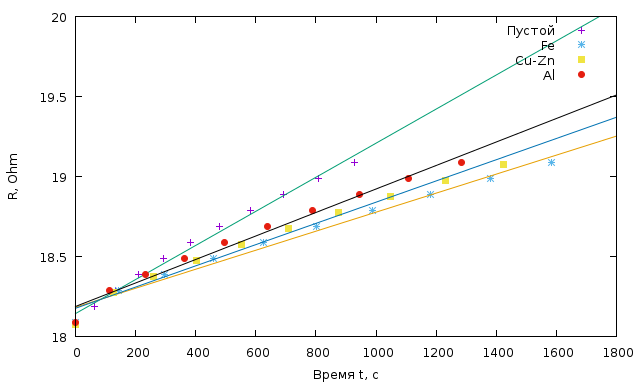
\includegraphics[height=90mm]{pic3.png}
		\caption{График зависимости сопротивления от времени}
	\end{figure}
	По графику при $R_k$:\\
	Калориметр: $\frac{dR}{dt}=10*10^{-4} \ \frac{\Omega}{c} \Rightarrow C_K' = 759,32\  \frac{\text{Дж}}{K}$ \\
	Железо: $\frac{dR}{dt}=6,67*10^{-4} \ \frac{\Omega}{c} \Rightarrow C_{Fe}' = 1139,66\  \frac{\text{Дж}}{K}$ \\
	Латунь: $\frac{dR}{dt}=6,94*10^{-4} \ \frac{\Omega}{c} \Rightarrow C_{Cu-Zn} ' = 1095,32\  \frac{\text{Дж}}{K}$ \\
	Алюминий: $\frac{dR}{dt}=7,48*10^{-4} \ \frac{\Omega}{c} \Rightarrow C_{Al}' = 1025,85\  \frac{\text{Дж}}{K}$ \\\\
	Теплоёмкость тел ($C=C'-C_k'$):\\
	$C_{Fe} = 379,7 \  \frac{\text{Дж}}{K}$ \\
	$C_{Cu-Zn} = 336,0 \  \frac{\text{Дж}}{K}$ \\
	$C_{Al} = 226,5 \  \frac{\text{Дж}}{K}$ \\
	\\Погрешности:\\
	$\sigma _t = 1 c,\  \sigma _R = 1.10^{-3} \Omega,\ \sigma _U = 0,1 V,\  \sigma _I = 0.01 A$ \\
	$\frac{\sigma _K}{K} = 0,02$\\
	$\frac{\sigma _C}{C} = 0,041$
	\begin{table}[h!]
 		\centering
	\begin{tabular}{|c|c|c|c|c|c|}
		\hline
		$C_{Fe}$ уд., $\frac{\text{Дж}}{K\cdot kg}$ & $C_{Fe}$ мол., $\frac{\text{Дж}}{K\cdot mol}$ & $C_{Cu-Zn}$ уд., $\frac{\text{Дж}}{K\cdot kg}$ & $C_{Cu-Zn}$ мол., $\frac{\text{Дж}}{K\cdot mol}$ \\
		\hline
		$466 \pm 19$ & $26 \pm 1$ & $386 \pm 16$ & $24 \pm 1$ \\
		\hline
		$C_{Al}$ уд., $\frac{\text{Дж}}{K\cdot kg}$ & $C_{Al}$ мол., $\frac{\text{Дж}}{K\cdot mol}$ &&\\
		\hline
		 $930 \pm 30$ & $24,8 \pm 0.8$ &&\\
		 \hline
    	\end{tabular}
  		\caption{Полученные результаты}
	\end{table}

	\paragraph{Вывод:}
	В ходе работы по опредлению теплоемкости твердых тел были опредлены теплоемкости по экстраполяции отношения $\frac{\Delta Q}{\Delta T}$ к нулевым потерям тепла.\\
	В эксперименте были определены удельные и молярные теплоемкости. В пределах погрешности результаты совпадают с табличными.
\end{document}